\documentclass[22pt]{beamer}
\usepackage[orientation=portrait, size=custom, width=91.44, height=60.96,scale=1.2]{beamerposter} % 36in*2.5 = 90cm
\usepackage[absolute,overlay]{textpos}
\usepackage{bookmark} %pdflatex says to use this to avoid errors...
\usepackage{graphicx} %for including images
\graphicspath{{assets/images/}} %location of images
\usepackage{wrapfig} %wrap text around the images
\usepackage{listingsutf8}    %package for code environment; use this instead of verbatim to get automatic line break; use this instead of listings to get (•)
\usepackage{amsmath}
\usepackage{gensymb}
\usepackage[export]{adjustbox}
\usepackage[skins,theorems]{tcolorbox}
\usepackage{tikz}
\newcommand*\circled[1]{\tikz[baseline=(char.base)]{
            \node[shape=circle,draw,inner sep=2pt] (char) {#1};}}
\usepackage{array}
\usepackage{booktabs,adjustbox}
\usepackage{subcaption}
\usepackage{pgfplots}
%plot options
\pgfplotsset{width=7cm,compat=1.8}
\PassOptionsToPackage{gray}{xcolor}
\usepackage{cite}
\usepackage{fancyvrb}

\usetikzlibrary{shapes,shapes.geometric,arrows,fit,calc,positioning,automata,}

\usepackage{wrapfig}

%\mode<presentation>
%this doesn't seem to make any difference; leave for now for trying out
\usetheme{Berlin}
\definecolor{MacBlue}{rgb}{0.10196,0.22353,0.53725}
\definecolor{MacMaroon} {rgb}{0.47843, 0, 0.23137}
\definecolor{MacMaroon2} {rgb}{0.47451, 0, 0}
\definecolor{MacGray}{rgb}{0.50196,0.49804,0.51765}
\definecolor{MacMaroon3}{rgb}{00.47,0.2,0.31}
\definecolor{MacGold}{rgb}{1, 0.75,0.35}
\usecolortheme[named=MacMaroon2]{structure}
\setbeamertemplate{caption}[numbered]
\setbeamertemplate{navigation symbols}{}

\title{A New Taxonomy of Software Testing Approaches}
\subtitle{Seeking More Standardized Standards}
  \author[Crawford]{Samuel Joseph Crawford\newline \small crawfs1@mcmaster.ca} % \{schankuc, geiskkod, smiths, anandc\}
  \institute[McMaster University]{Department of Computing and Software, McMaster University} % $^\dagger$
  \date{April 22, 2023}

\begin{document}
%compile with pdflatex

%there is only one frame, because there is only one page; yeah, it's a poster
%textblock and block seem to work nicely to organize layout
\begin{frame}[fragile]

    \begin{textblock}{2}(0.7,1)
        
\includegraphics[height=8.5cm]{eng_logo.png}
    \end{textblock}

    \begin{textblock}{2}(13,0.55)
        
\includegraphics[height=12.5cm]{cas_logo.png}
    \end{textblock}

    \begin{textblock}{8}(4,1)
        \titlepage
    \end{textblock}

    \begin{textblock}{7.25}(0.5,3.9)

        %this needs help
        \begin{block}{\fontsize{37}{20}\selectfont Background}
            \textit{McMaster Start Coding} and \textit{STaBL Foundation}'s mission is to uplift underprivileged
            youth by equipping them with 21st-century skills like coding. We have taught lessons to over
            30,000 students in the past seven years. We have found creating video games to be particularly
            engaging. We have developed and tested tools such as the state diagram tool
            \cite{pasupathi2022teaching}, which has been applied successfully by Grade 4-12 and 1st-year
            students to create single player games. The previous attempt, PAL \cite{schankula2020newyouthhack}, at creating a
            multiplayer game / app framework proved too complicated to be reasonably used by students. TEASync
            is a simplified framework allowing students to create multi-user applications.
            \vspace{5mm}
        \end{block}

        \begin{block}{\fontsize{37}{20}\selectfont Background: The Elm Architecture}
            \begin{itemize}
                \item Elm is a pure, strictly-typed functional programming language
                \item Every Elm program follows a rigid structure known as \textit{The Elm Architecture} (TEA)
            \end{itemize}
            % \begin{figure}
            %     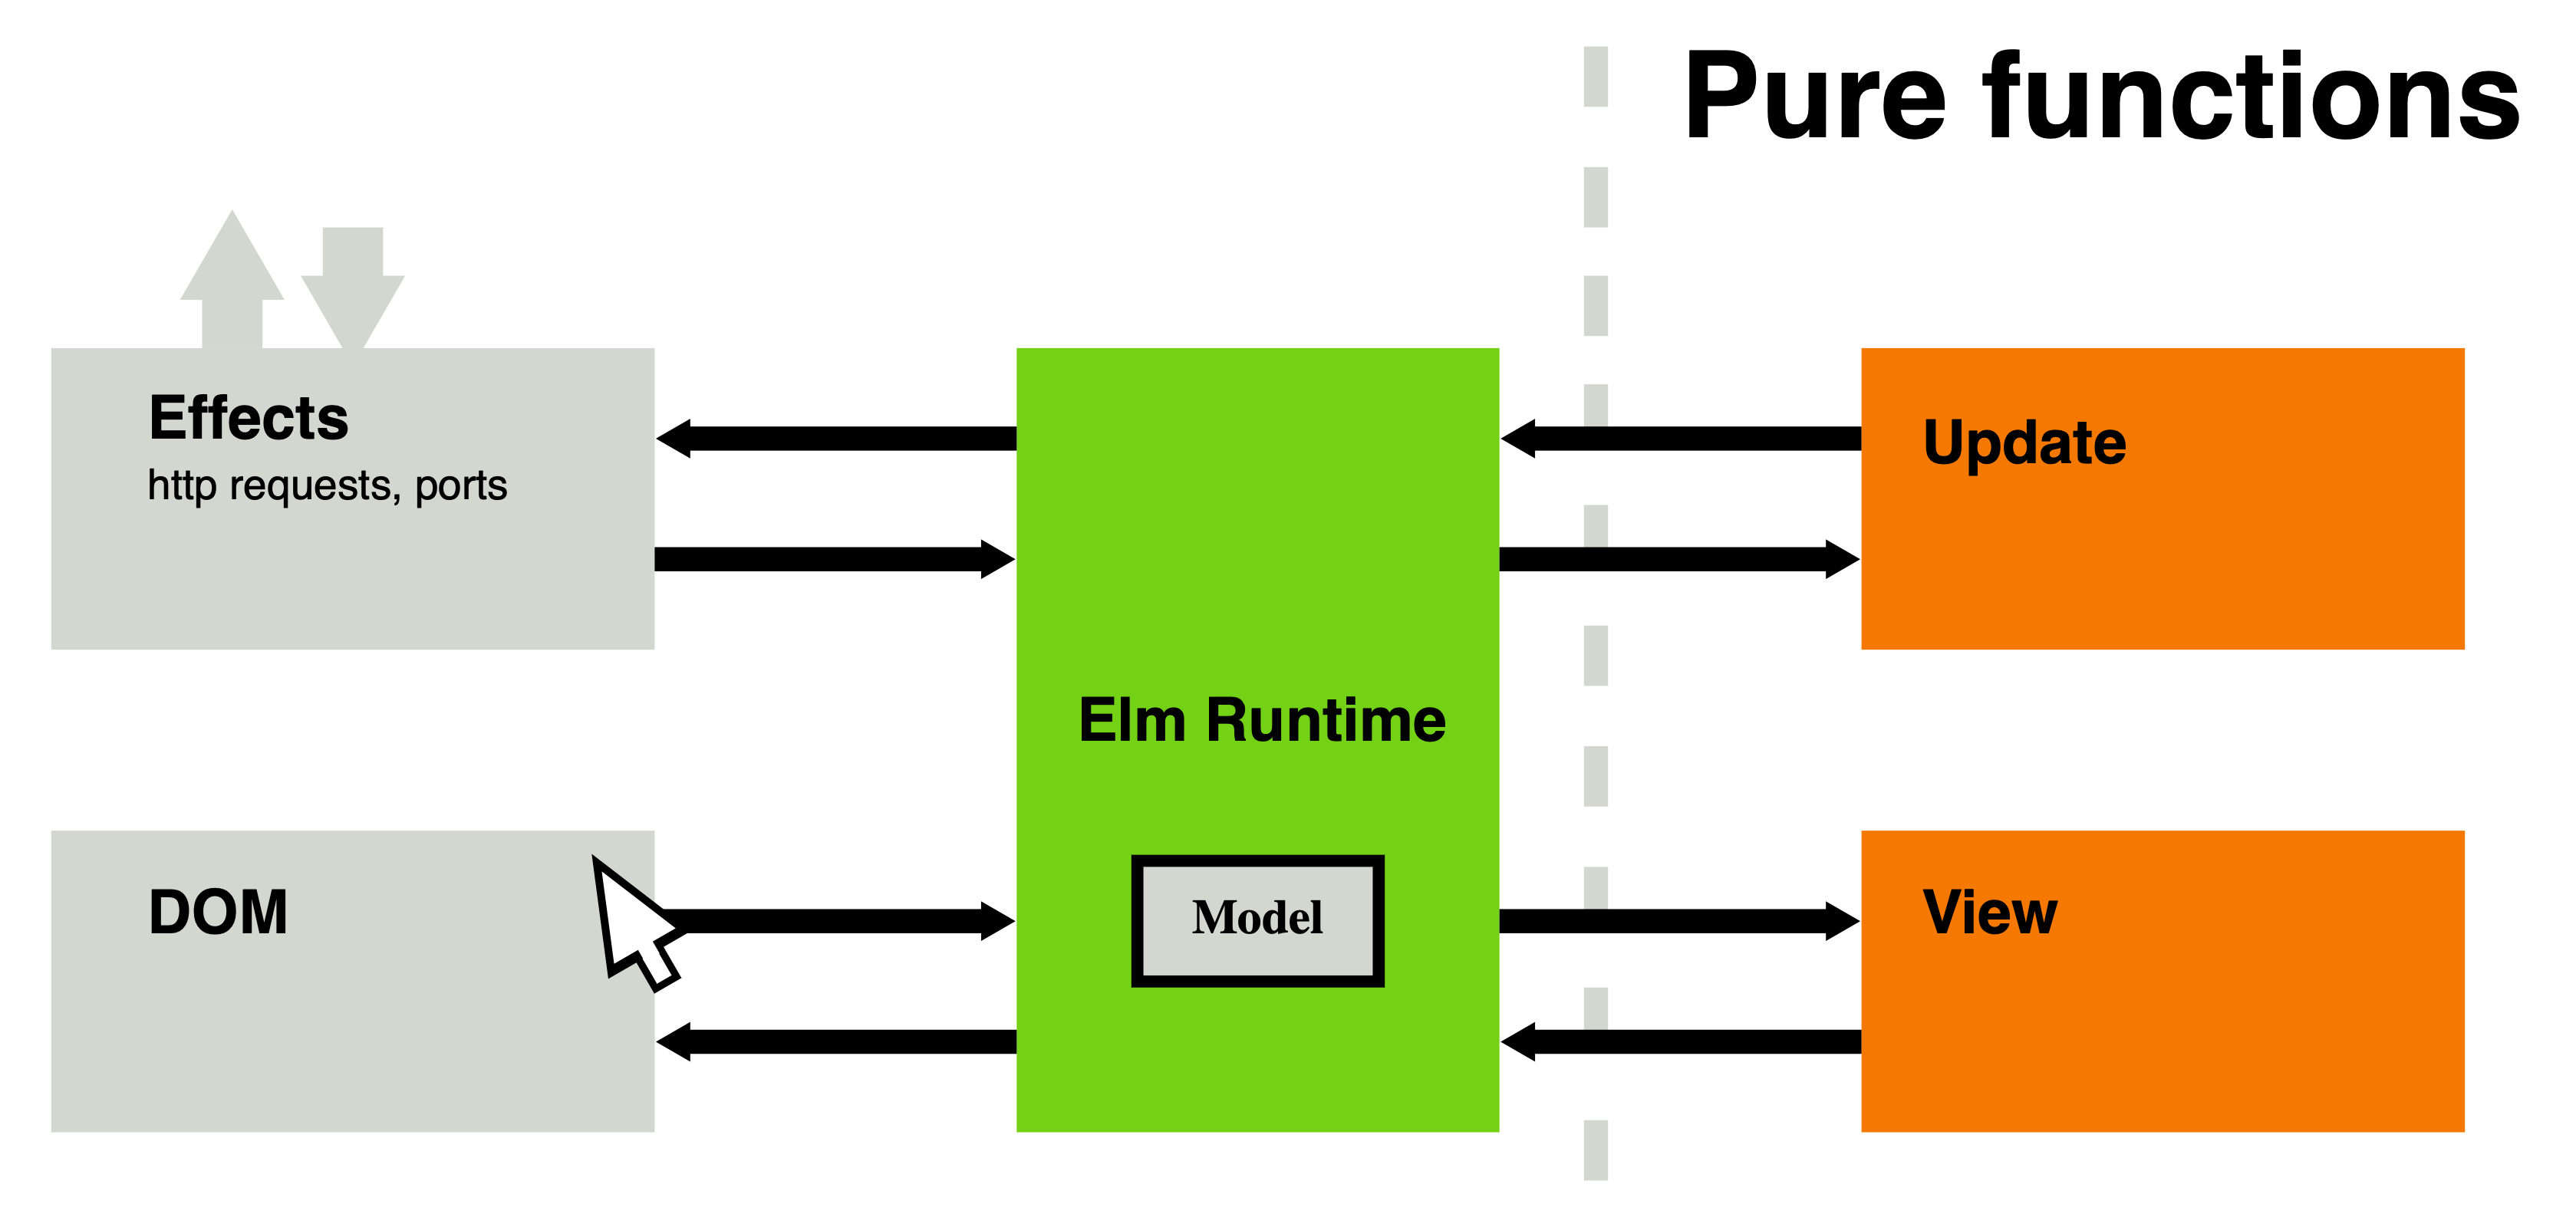
\includegraphics[height = 13cm]{TheElmArchitecture.png}
            %     \caption{The Elm Architecture consists of a \textit{model}, representing application data, a pure \textit{update} function to change the model in reaction to user events, called
            %         messages,
            %         and a pure \textit{view} function to render the application to the screen.}
            %     \label{Fig:TEA}
            % \end{figure}
            \vspace{-6mm}
        \end{block}

        \begin{block}{\fontsize{37}{20}\selectfont Theory: Extending The Elm Architecture to Multiple Clients}
            \begin{itemize}
                \item Theorem 1: Two clients running Elm programs having an identical initial model,
                      identical update functions, and processing an identical sequence of messages will end up
                      with an identical model.
                \item Proof: This can be shown easily by using Elm's pureness property.
                \item Corollary: Any number of Elm clients having an identical initial model,
                      identical update functions, and processing an identical sequence of messages will end up
                      with an identical model.
                \item Observation: By ensuring every client receives the same messages in the same order,
                      we effectively have a multi-user application, without writing any application-specific server
                      code.
            \end{itemize}
        \end{block}

        \begin{block}{\fontsize{37}{20}\selectfont TEASync Framework Architectural Overview}
            % \begin{figure}
            %     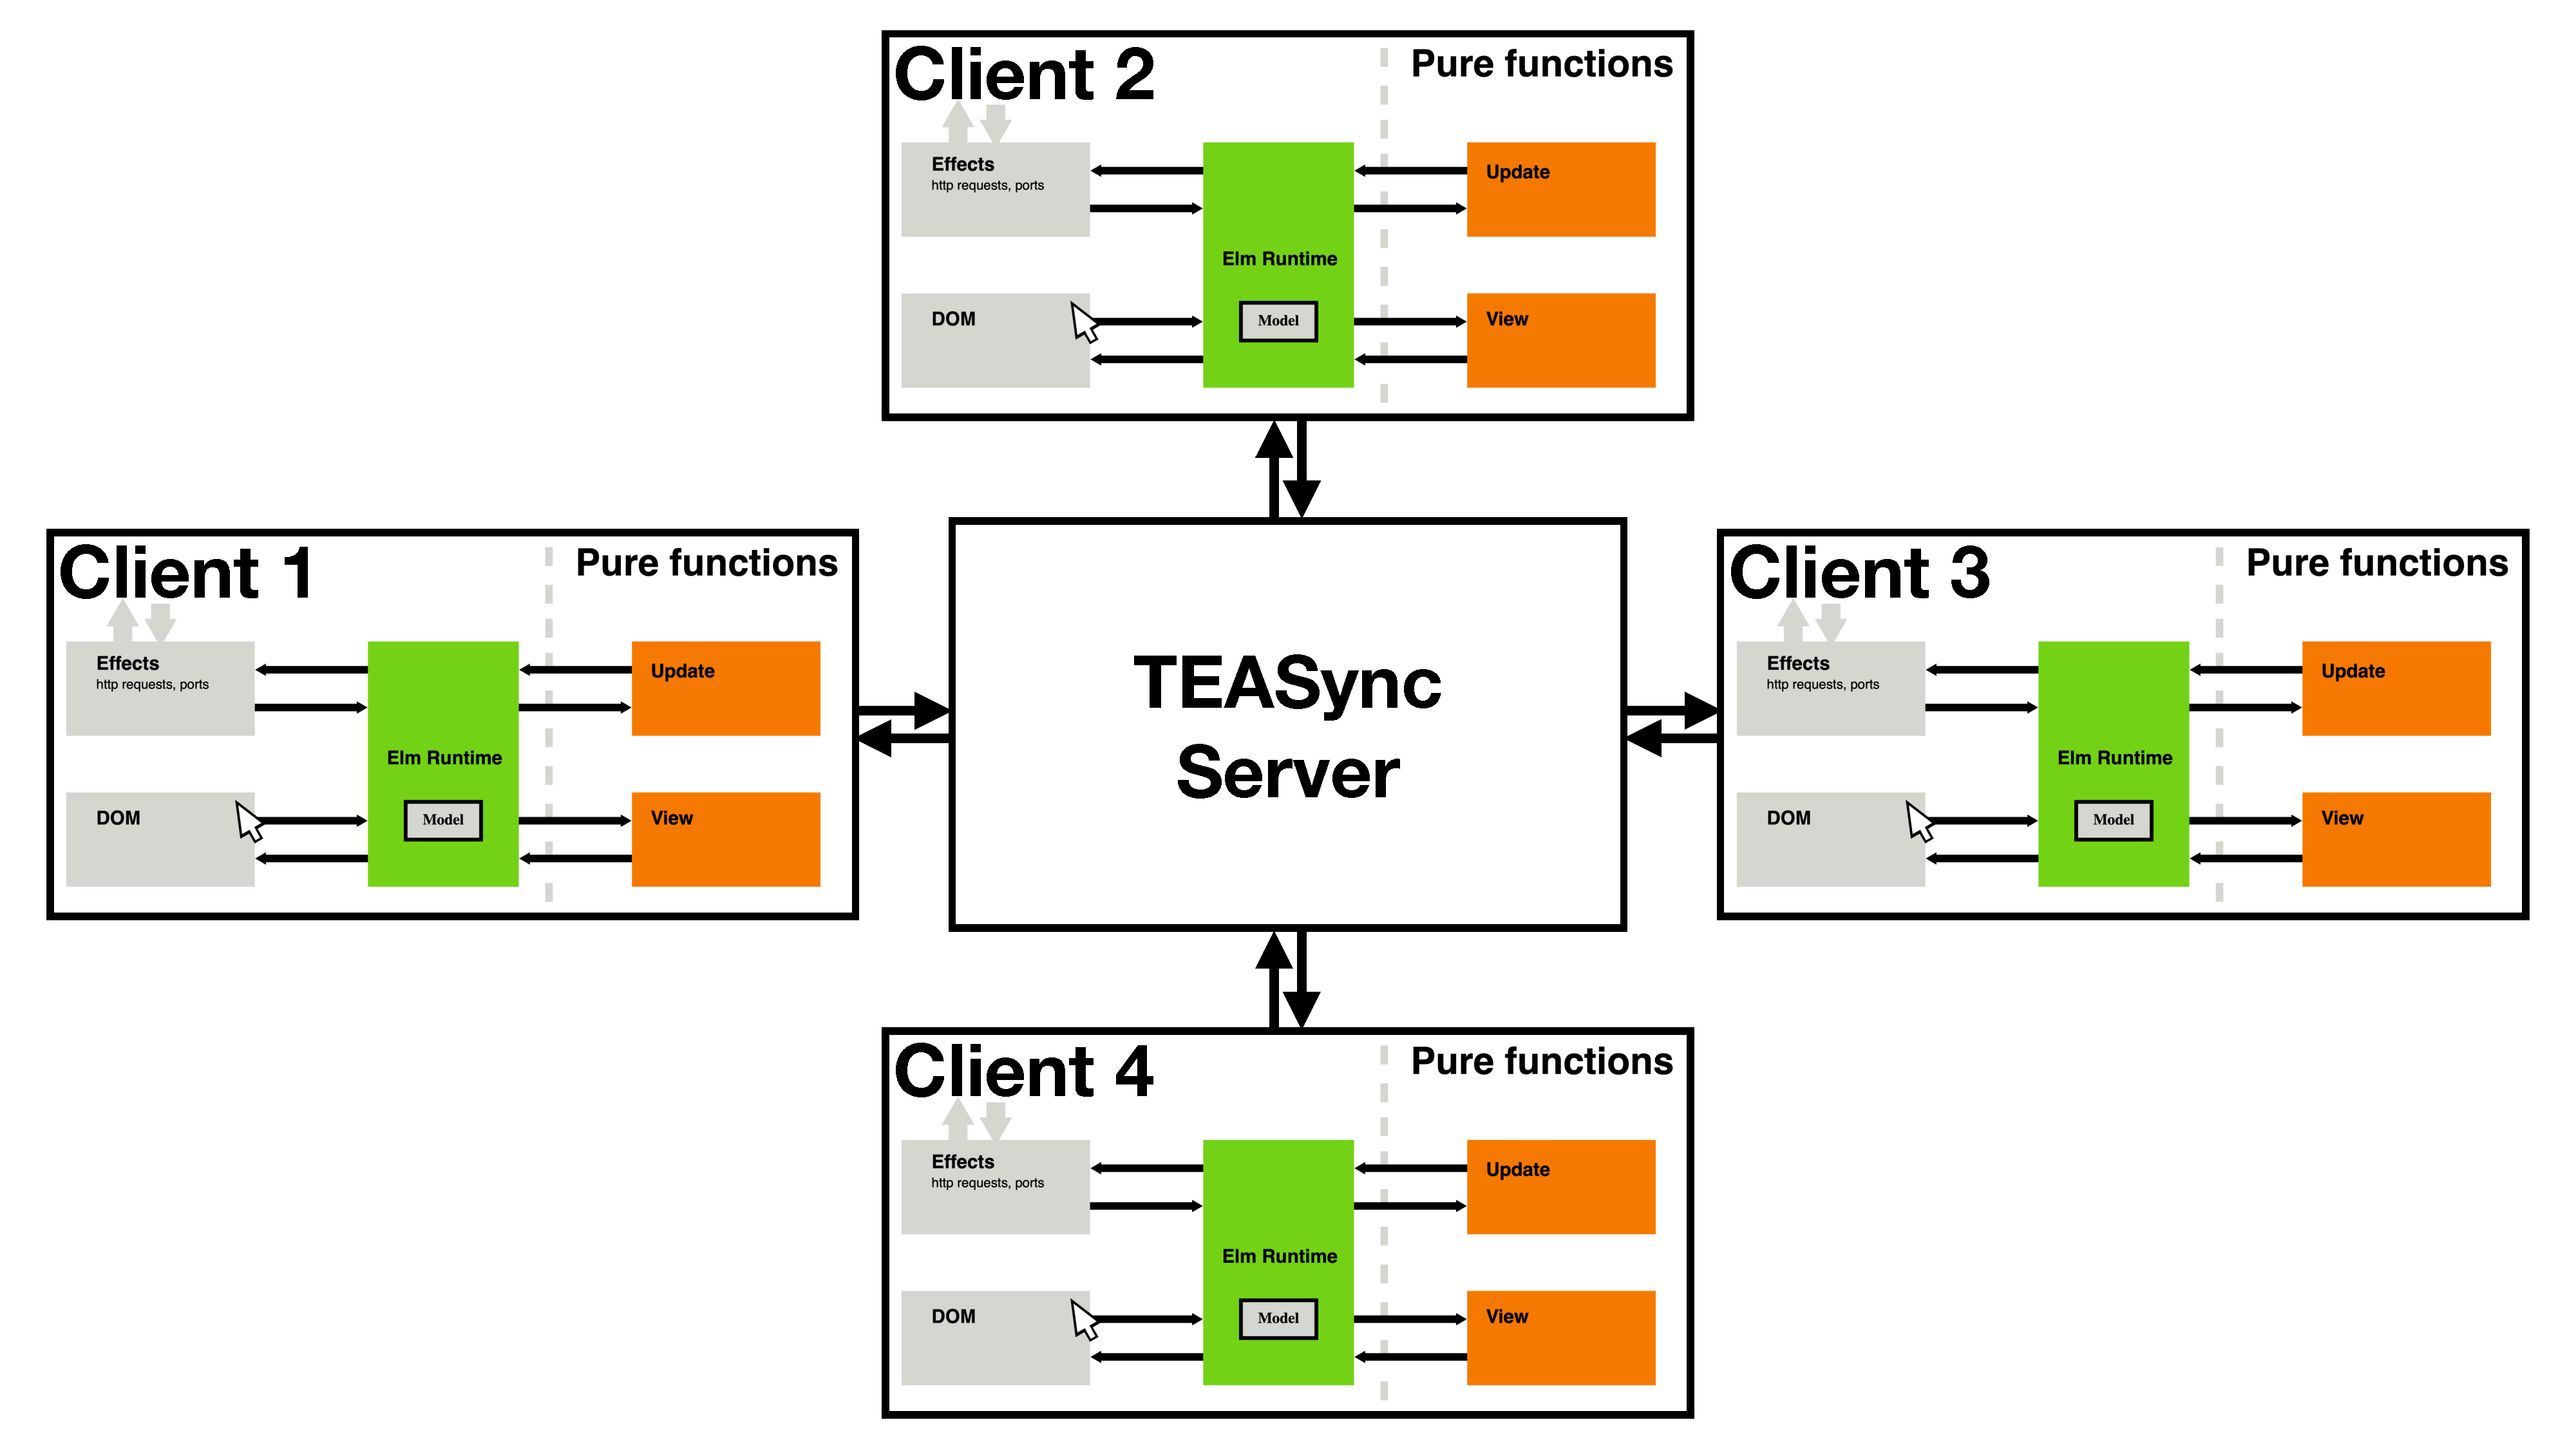
\includegraphics[height = 20cm]{figs/TEASyncDiagram.pdf}
            %     \caption{An example multi-user application with four concurrent clients. TEASync uses a generalized server written using the Integrated Haskell Platform (IHP)
            %         to synchronize all clients. The programmer writes no app-specific server-side code; rather they write only Elm code,
            %         greatly simplifying the process of creating a multi-user application. The TEASync framework handles
            %         communication and ensures that the ordering of messages is consistent for every client.}
            % \end{figure}
            \vspace{-6mm}
        \end{block}
    \end{textblock}

    \begin{textblock}{7.25}(8.25,3.9)
        \begin{block}{\fontsize{37}{20}\selectfont Example Applications}
            The following is a simple application which allows multiple users to increment and decrement an
            integer. Figure \ref{Fig:Counter} shows an example UI for this application. Figure \ref{Fig:Pong} shows an example Pong game made using this framework.

            \begin{Verbatim}
                type GlobalMsg = Increment | Decrement

                type alias GlobalModel = { count : Int }

                globalUpdate : GlobalMsg -> GlobalModel -> GlobalModel
                globalUpdate msg globalModel =
                case msg of
                Increment -> { globalModel | count = globalModel.count + 1 }
                Decrement -> { globalModel | count = globalModel.count - 1 }
            \end{Verbatim}

            % \begin{figure}
            %     \begin{subfigure}{0.49\textwidth}
            %         \centering
            %         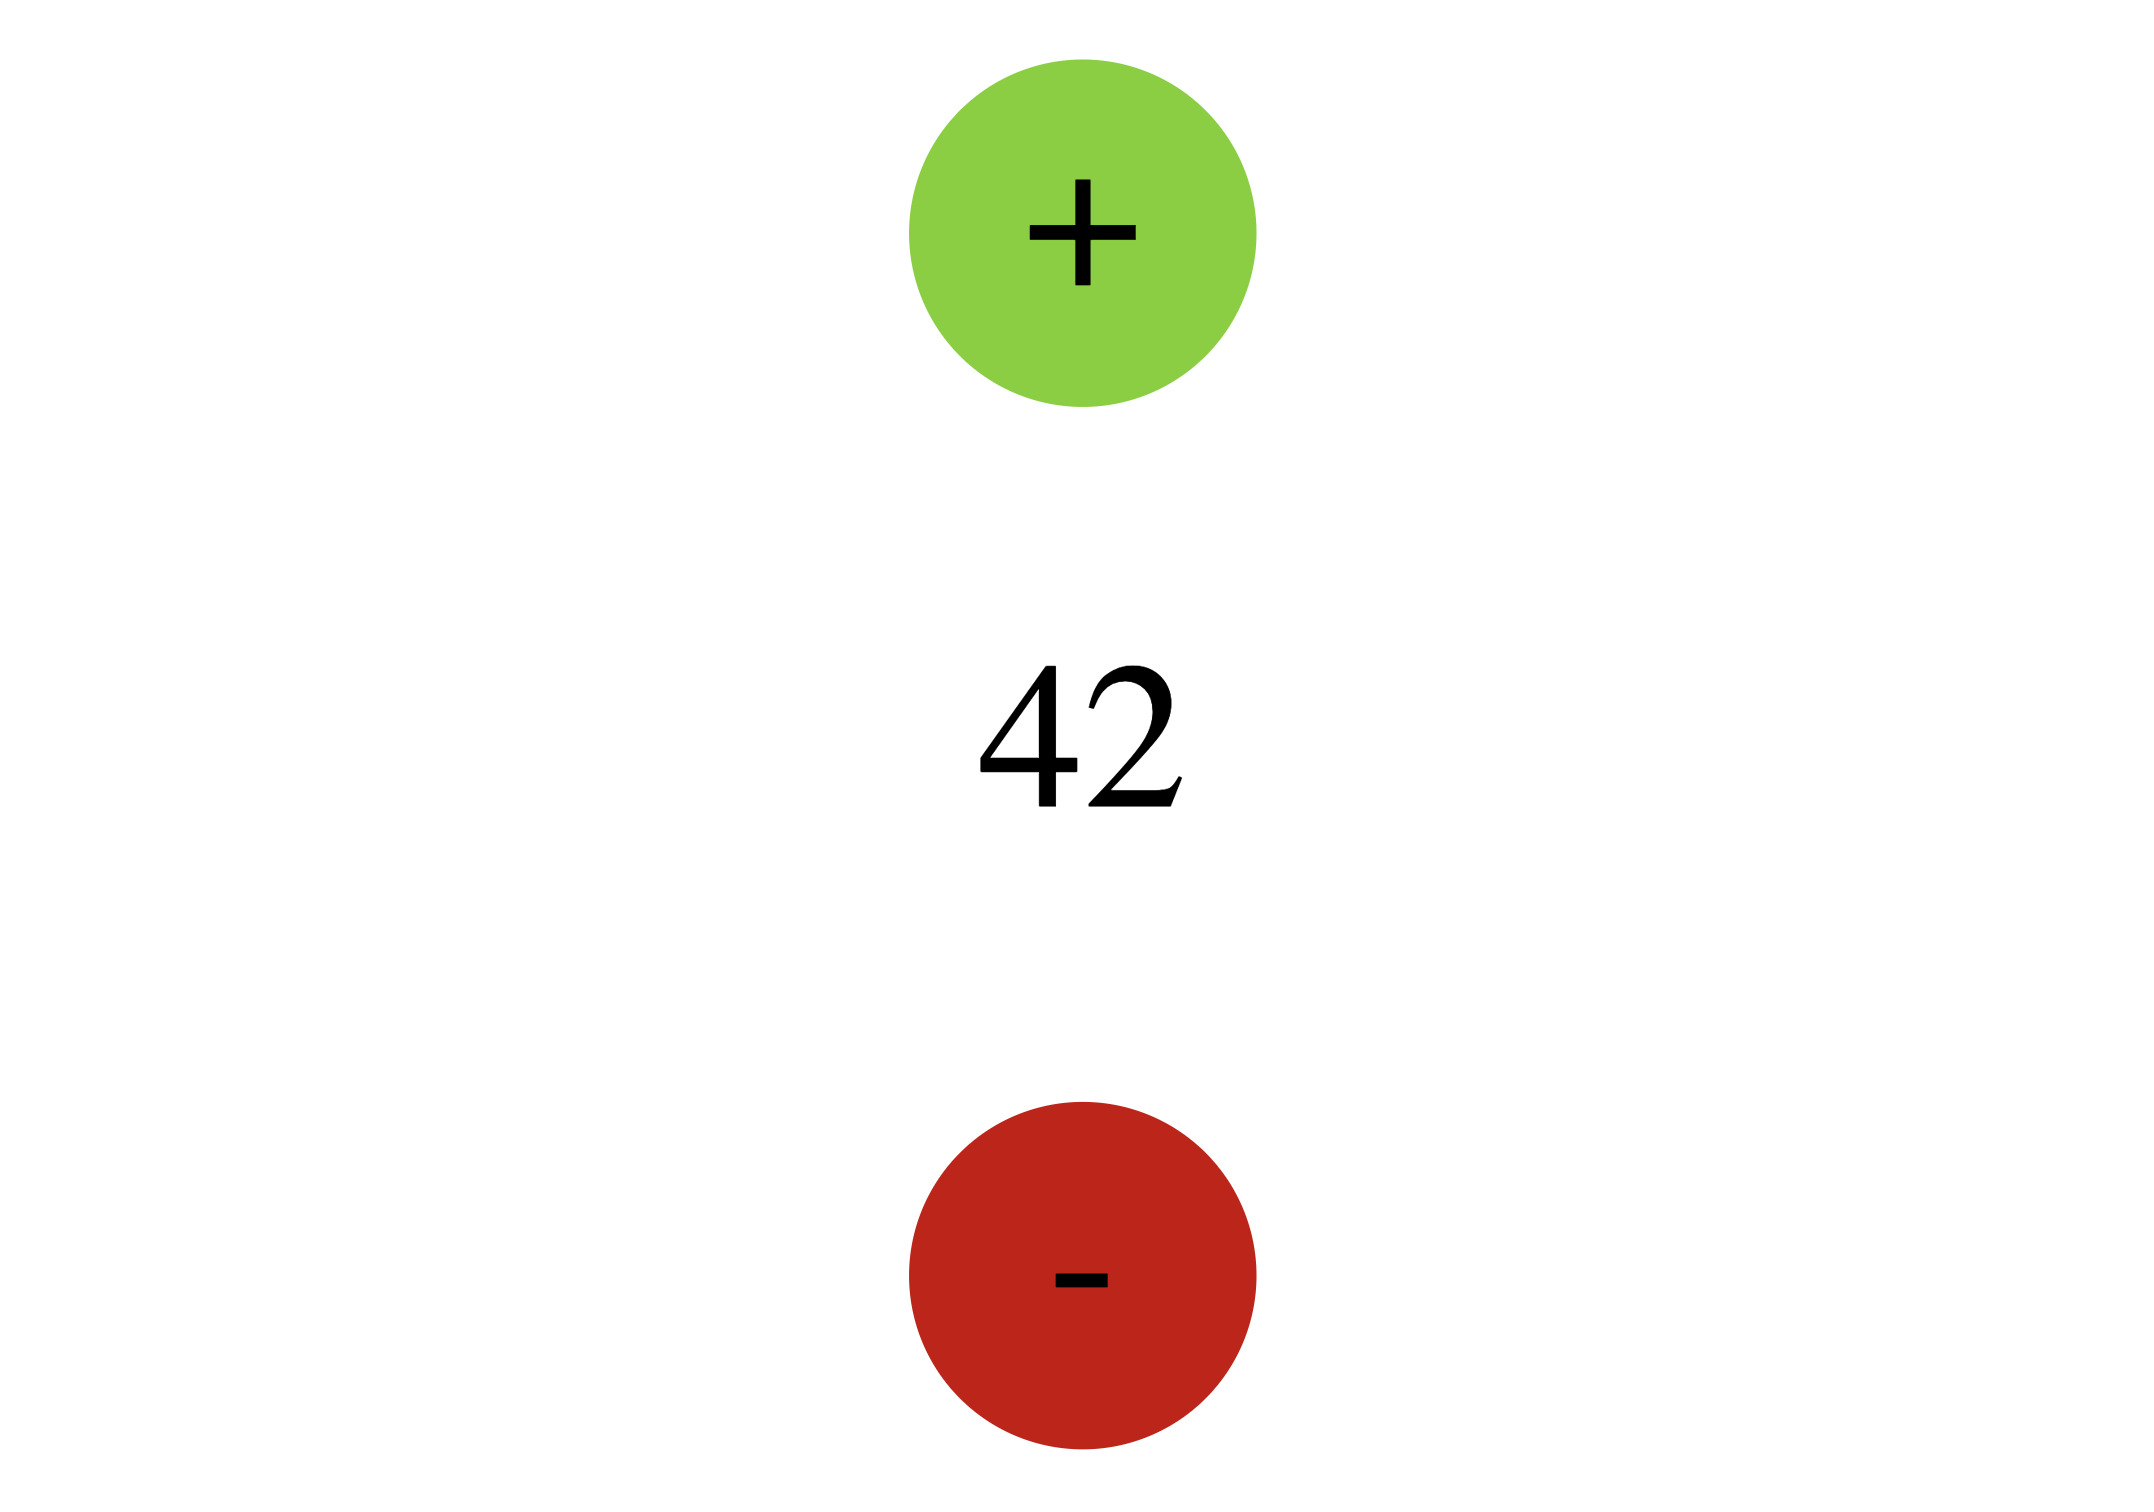
\includegraphics[height = 13.5cm,trim={0 5mm 0 5mm},clip]{IncDec.png}
            %         \caption{Example TEASync counting application}
            %         \label{Fig:Counter}
            %     \end{subfigure}
            %     \begin{subfigure}{0.49\textwidth}
            %         \centering
            %         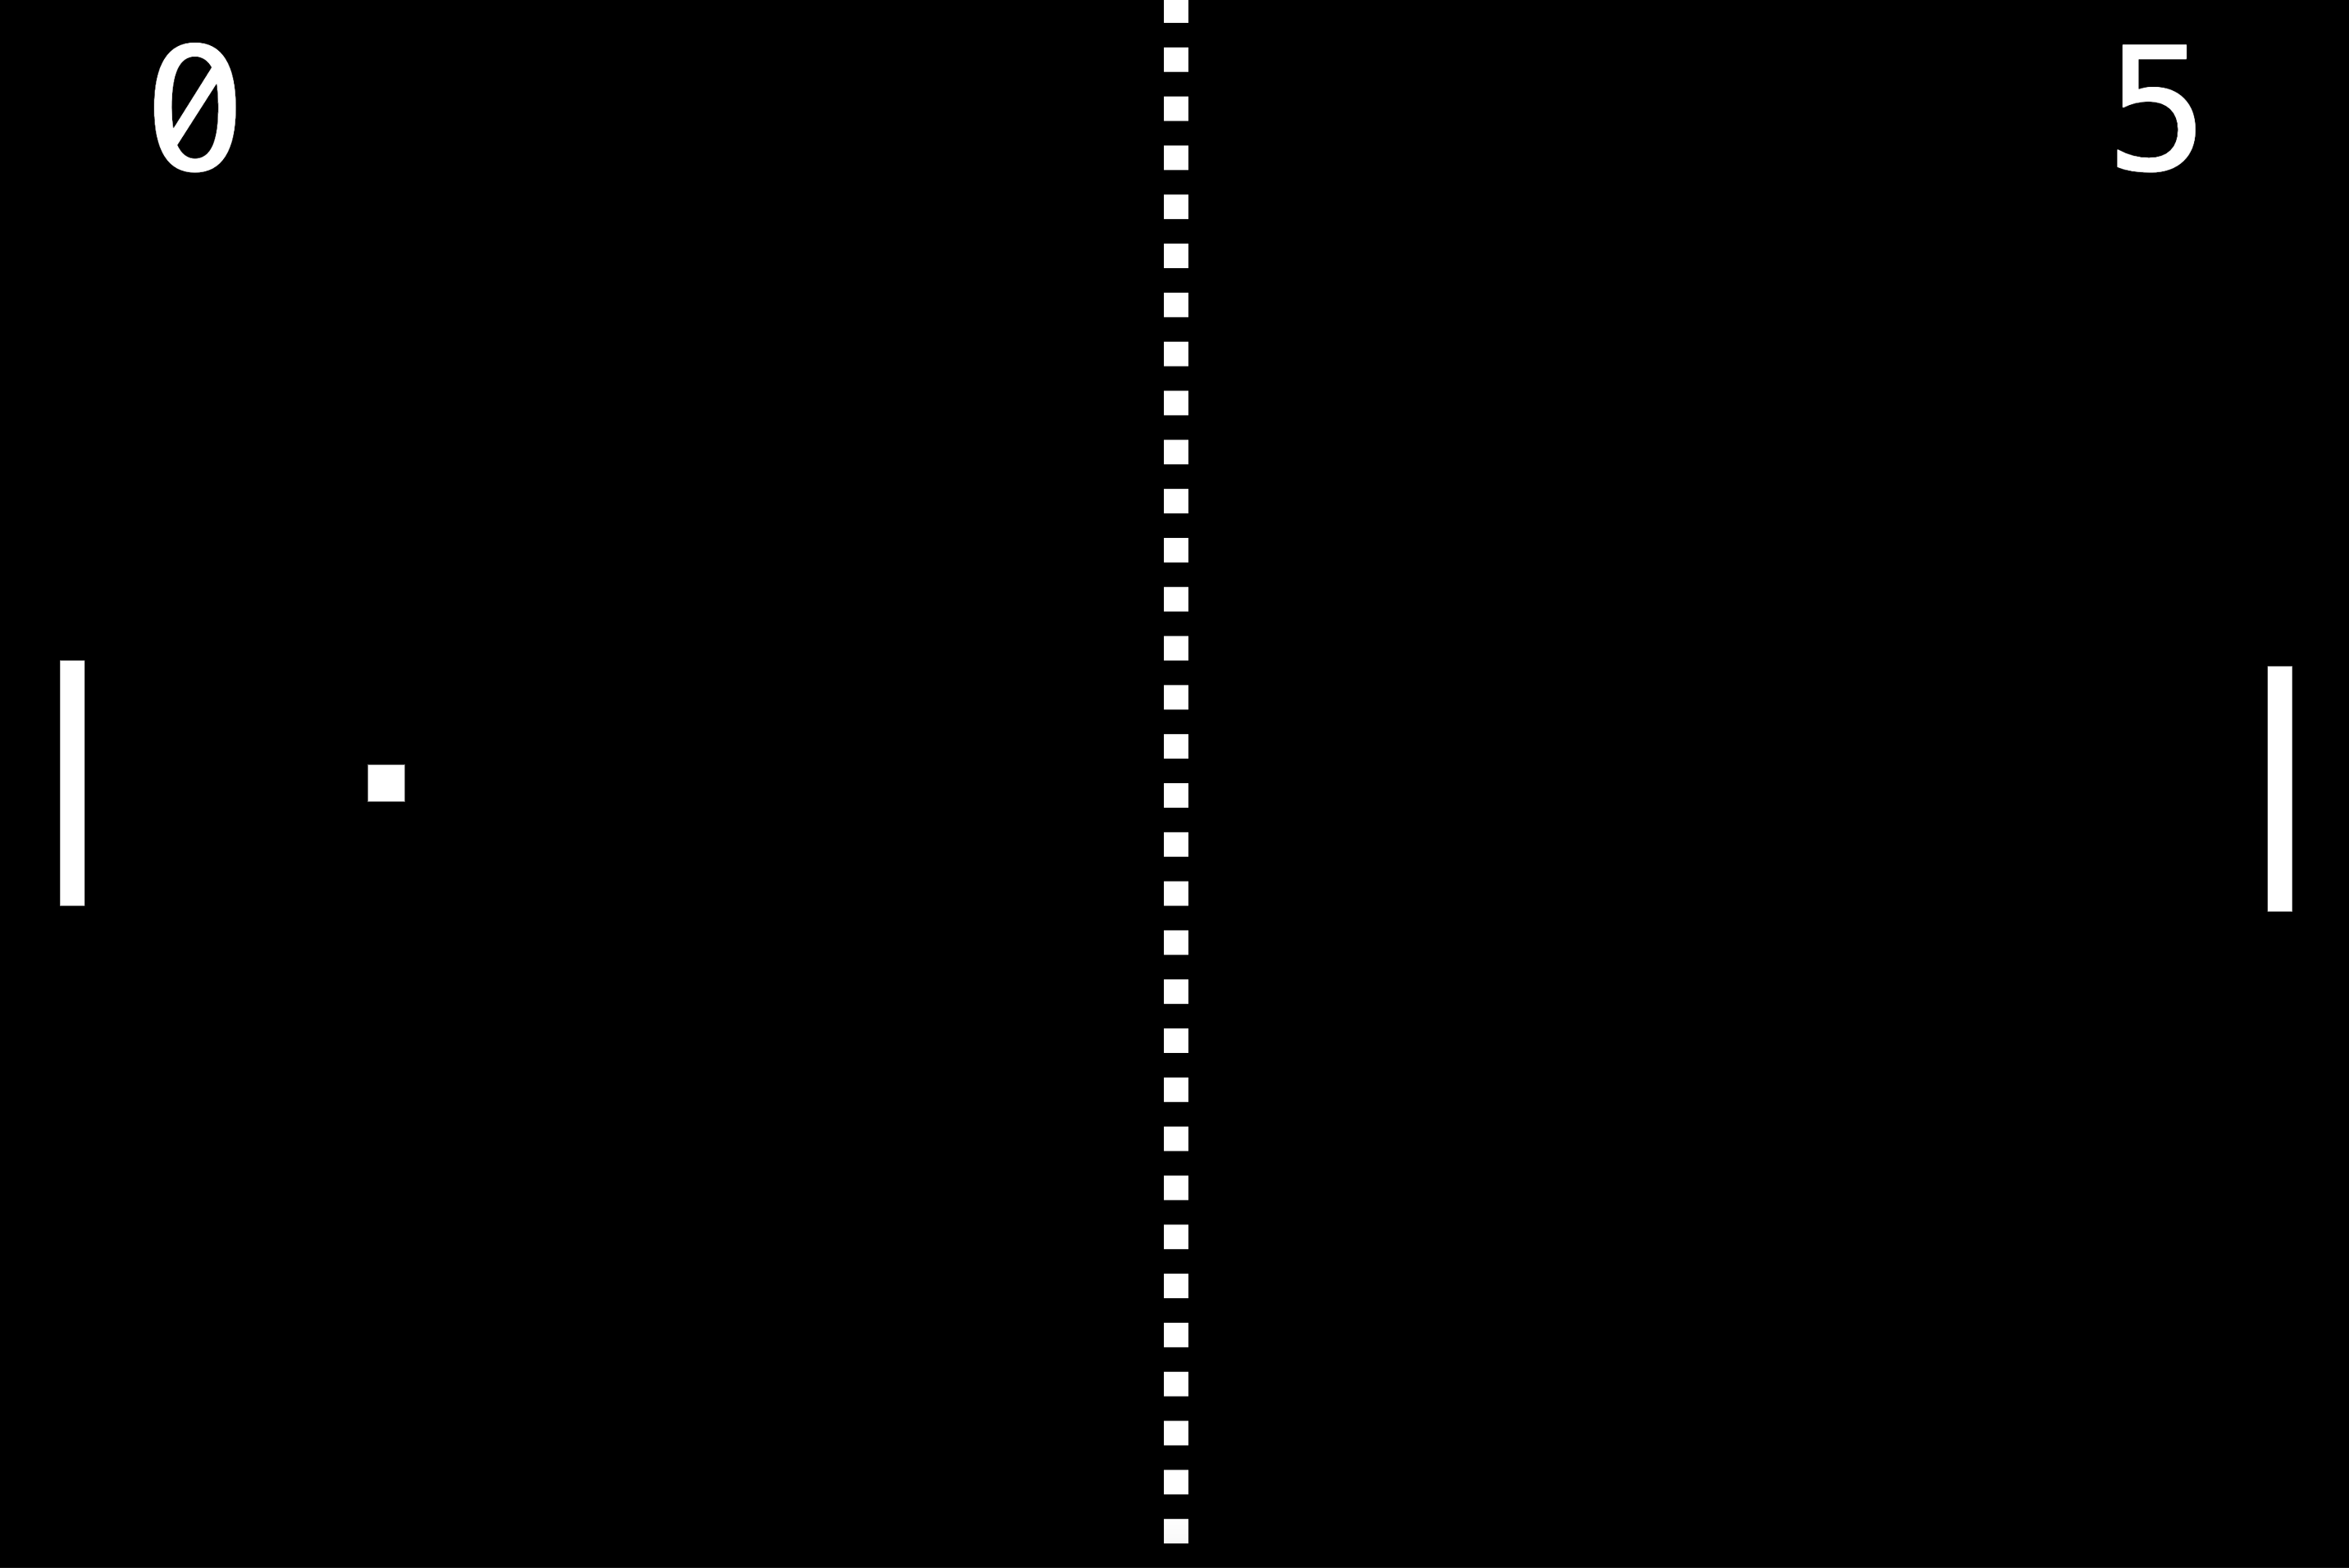
\includegraphics[height = 13.5cm]{Pong.png}
            %         \caption{Example TEASync multiplayer Pong game}
            %         \label{Fig:Pong}
            %     \end{subfigure}
            %     \caption{Example TEASync application user interfaces}
            % \end{figure}
            \vspace{-5mm}
        \end{block}

        \begin{block}{\fontsize{37}{20}\selectfont Conclusions \& Future Work}
            Leveraging the strictly-typed nature of Elm and its model-view-update architecture, we were able
            to create a simplified multi-user framework, requiring the programmer to write no server-side code. In addition to the upcoming pedagogical study, future work includes a data modelling extension allowing persistent, structured data, an
            authentication/authorization scheme, a binary data format to reduce network communication, and
            curriculum development for a TEASync-based summer camp.
        \end{block}

        % \begin{block}{\fontsize{37}{20}\selectfont References}
        % \scriptsize
        % \bibliographystyle{ieeetran}
        % \bibliography{bib}
        % \end{block}

        \begin{block}{\fontsize{37}{20}\selectfont References}
            \setbeamertemplate{bibliography item}{\insertbiblabel}
            \bibliographystyle{ieeetr}
            {\scriptsize
                \bibliography{bib}}
        \end{block}

        \begin{block}{\fontsize{37}{20}\selectfont Acknowledgments}
            We thank NSERC for CGS-M funding and the Government of Ontario for OGS funding.
        \end{block}

        % \begin{figure}[htbp]
        %     \centering
        %     
\includegraphics[height=5cm,trim={0 0 28.5cm 0},clip]{nserc-logo.jpg}
        %     \hspace{0.5cm}
        %     
\includegraphics[height=5cm,trim={16.5cm 0 0 0},clip]{ontario@2x-print.png}
        %     \hspace{0.5cm}
        %     
\includegraphics[height=5cm]{STaBLLogoWS.png}
        %     \hspace{0.5cm}
        %     
\includegraphics[height=5cm]{elm-logo.png}
        %     \hspace{0.5cm}
        %     
\includegraphics[height=5cm]{IHPLogo.png}

        % \end{figure}
    \end{textblock}

    % \begin{textblock}{5}(10.7,3.8)
    % \begin{figure}
    % 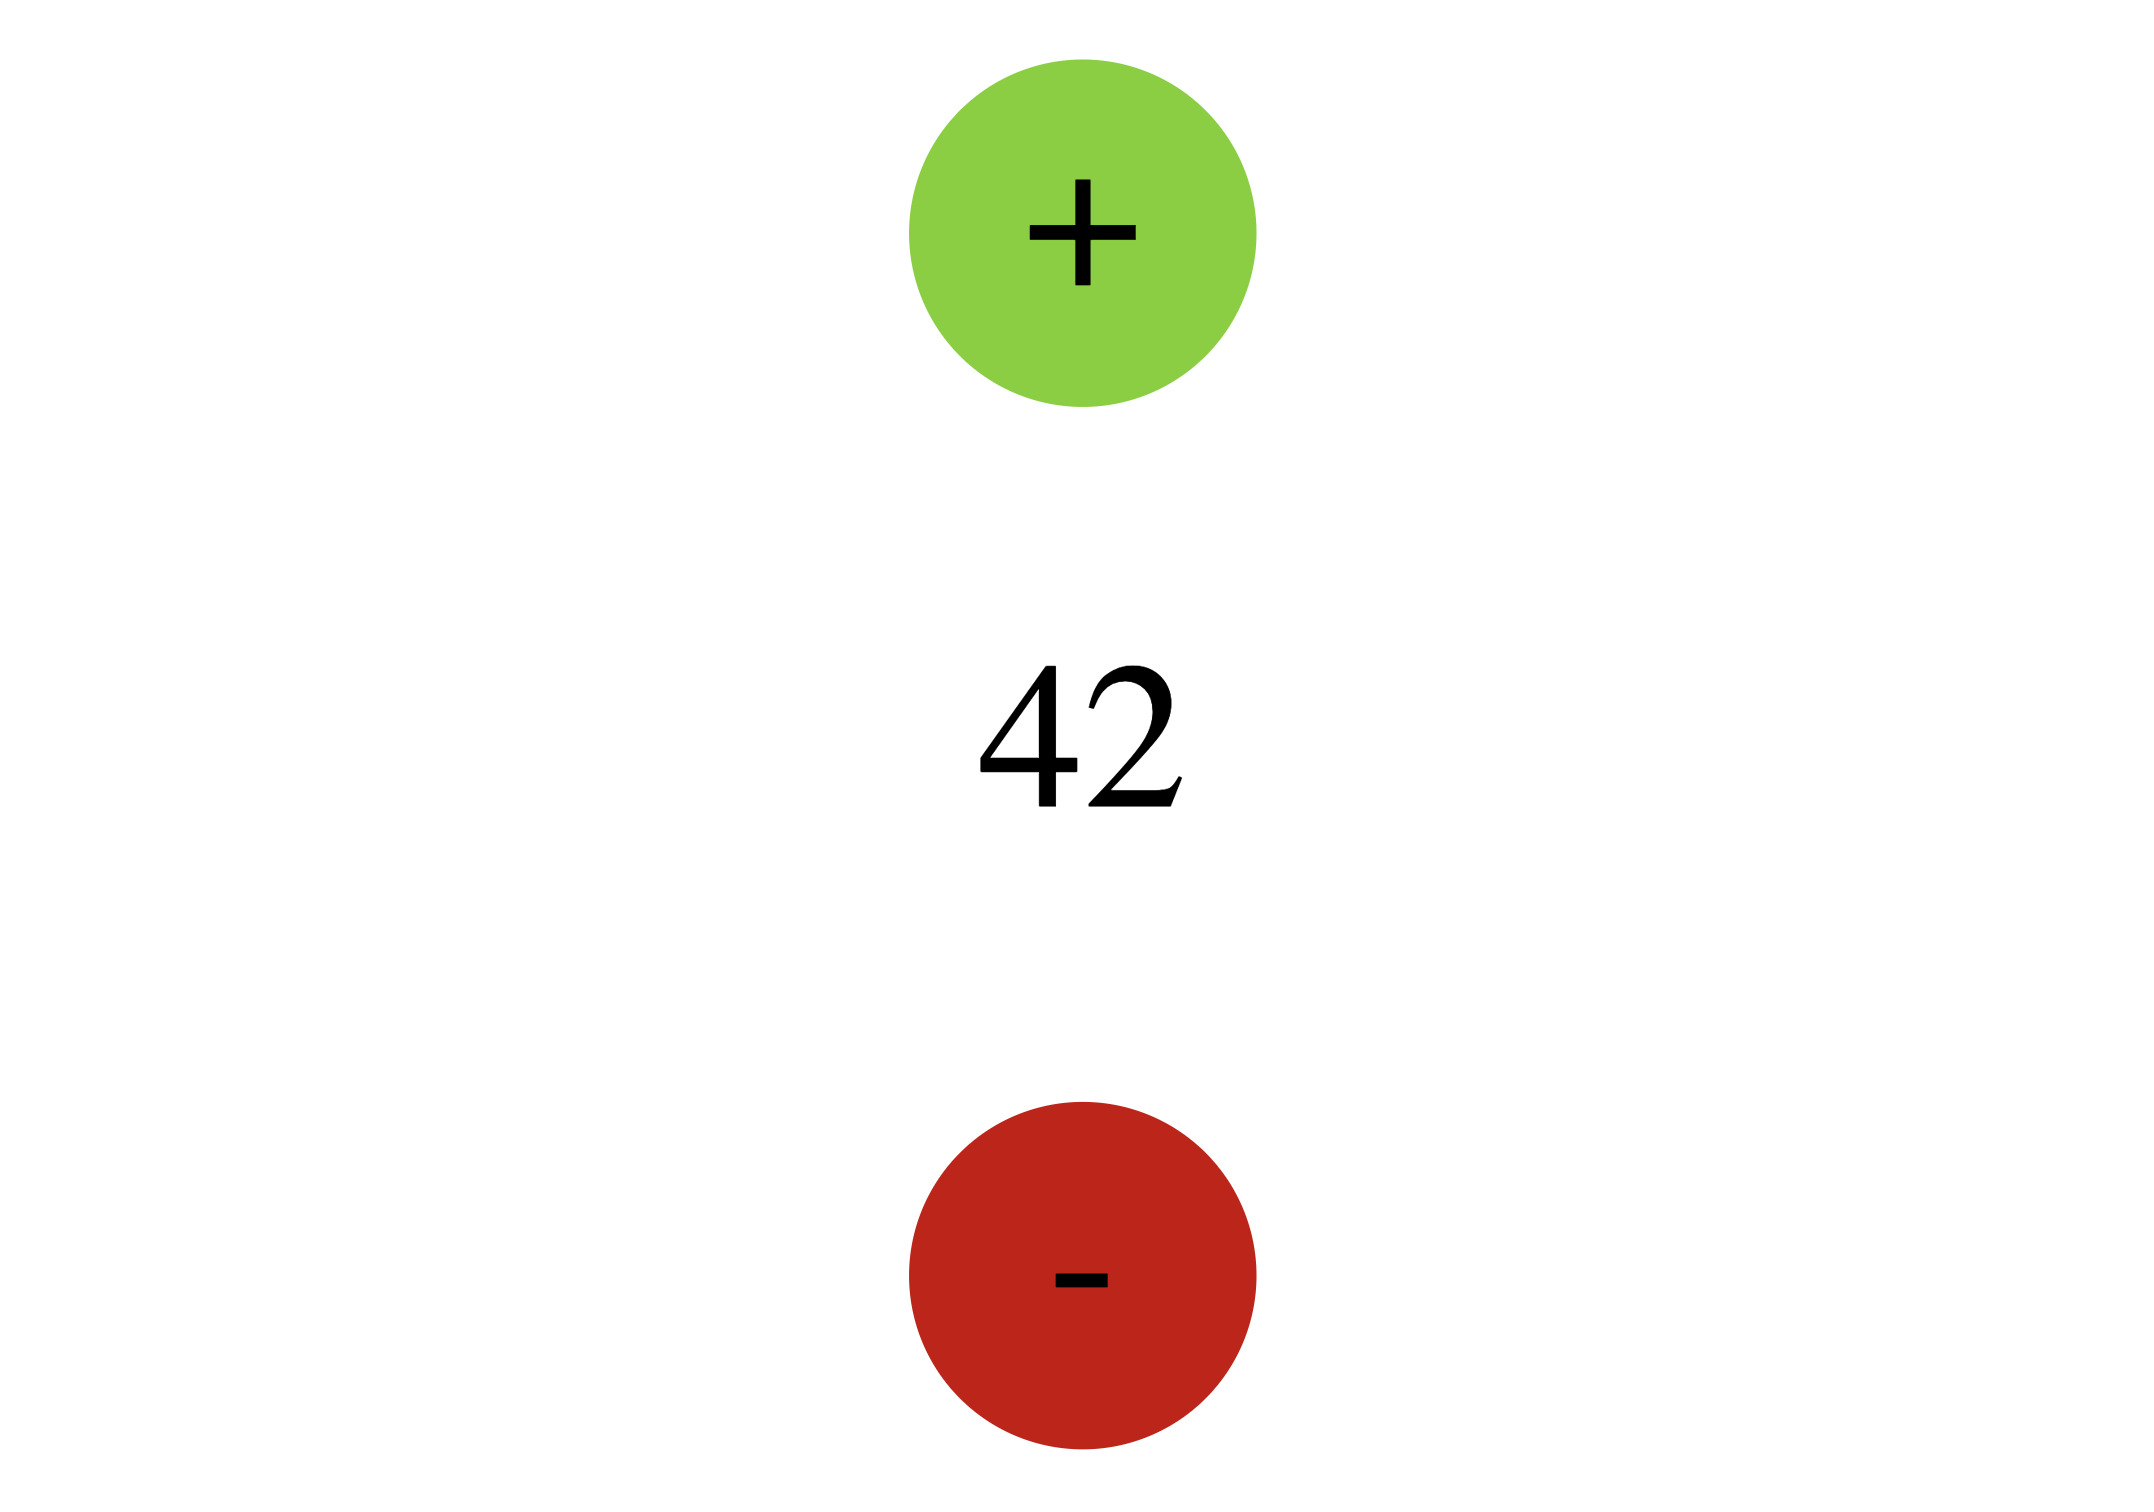
\includegraphics[height = 11cm]{IncDec.png}
    % \caption{Example TEASync counting application}
    % \label{fig:Counter}
    % \end{figure}
    % \end{textblock}

\end{frame}
\end{document}
